\chapter{Context} \label{context}
People have always wanted to stay in contact with one another. Since the introduction of the internet it has never been so easy, at first we used primarily email for communication with one another over the internet, but this was a technology adapted from letters. Early social media examples can be found in early instant messengers like MSN Messenger \cite{historyofsocialmedia} which allowed the user to instantly communicate with one another across the world. But instant messenger platforms would be rapidly be replaced by other more robust sites such as Facebook(2004), Flickr(2004), Bebo(2005) and MySpace(2005) \cite{historyofsocialmedia} to name a few. These sites revolutionized how we communicate today by giving us an online presence that others can use to find and communicate with us.

% ========================== Early Electronic Communication  ========================== 
\section{Early Electronic Communication}
Early on, when the internet was just starting off it was used to connect universities and colleges together and was known as the ARPANET \cite{historyofmedia}. ARPANET allowed 3rd level institutions to communicate with one another through this new means of communication by linking their computers together to create the first usable computer network over a long distance. This evolved quickly, adding more universities, colleges, and research centers. This early form of communication was used to share research data between these institutions, which was seen as a great tool for the scientific method of sharing research and reading others in order to come to a conclusion. \cite{historyofinternet}

ARPANET quickly evolved into the internet we know today. As the internet progressed from a relatively small network between 3rd level institutions and research centers, to slowly entering peoples houses where everyone could connect to this one network. Early internet used telecommunications lines and shared bandwidth with phones. Although this was a great way of getting the internet into peoples houses quickly by using the infrastructure already in place, this created a problem where you could either use the phone or the internet as you had to use the phone line to dial up the internet. This created a problem where the speed was too slow and any interruption such as using the phone to call someone. This stage of internet infrastructure was called dial-up. Dial-up was extremely slow with a maximum speed of 56Kbit/s, this slow speed and shared cable with a phone line made instant messaging slow and not very viable. For example, a 2GB file that today is a relatively small file would take 3 and a half days to download without interruption at the maximum speed and the maximum speed was rarely met and retained for most users. \cite{historyofinternet}

During this era emails were the main method of communication, it was text only and didn't require the user to be on their PC when the user sends the email. Email during this time was easy for users to understand during the early stage of home computers as it was just an electronic letter or e-mail. This allowed people of all ages to quickly grasp this new technology. And although emails would last well into the present their preference to communicate with friends and family would be replaced, and emails would be used in a more professional environment such as 3rd level institutions and the workplace. \cite{historyofsms}

% ========================== Rise of Social Media  ========================== 
\section{Rise of Social Media}
Social media started in the late '90s but was a very early stage and was missing features that we consider standard today. These social media applications were centred around messaging applications such as AOL Instant Messenger(1997), MSN Messenger(1999) and Yahoo! Messenger(1999). These applications were extremely popular among the younger population replacing email for the most part for this younger generation. These applications created a standard among social media sites to come by offering an instant messenger to entice on their application to move onto the new competitors.

\begin{figure}[!htb]
  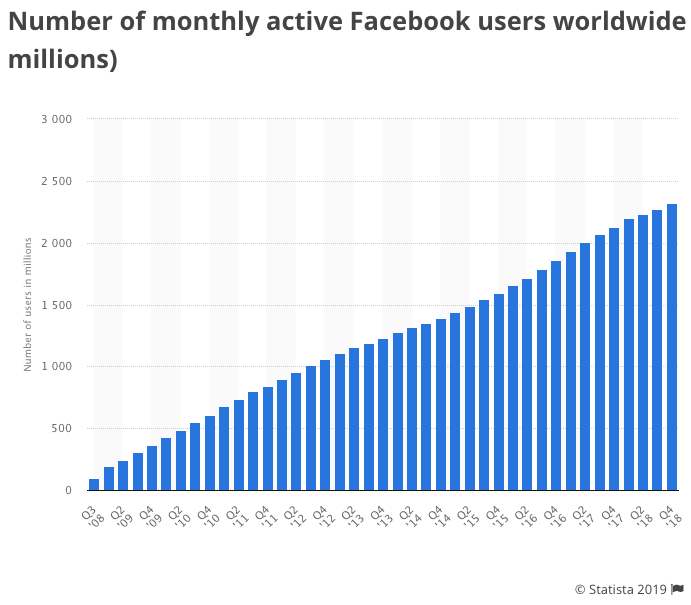
\includegraphics[width=\linewidth]{img/facebook-growth.png}
  \caption{Facebook Growth}
  \label{fig:FacebookG}
\end{figure}

In early 2000 is the year social media sites we know today started out and came into their own. Sites such as Facebook(2004), Reddit(2005) and Twitter(2006) all launched in the early '00s and are still very active today. These sites quickly gained an audience from people who wanted a more involved experience. These sites offered profile pages the user could customize and have users interact with one another. Facebook, for example, is the most popular social media site today (2019) expanding year over year in terms of users. \cite{historyofsocialmedia}

Facebook has remained relevant through expanding it's market and language options to make it more inclusive for people outside the western hemisphere where it first took off. which allowed it to incrementally increase its user-base year over year.

Sites early on like MySpace(2003), Flickr(2004) and Bebo(2005) all gained traction but rapidly fell out of use once more competition came into the market such as Facebook and Twitter. These early social media sites were generally popular with the younger generation but as more robust social media sites came into the light they fell out of use. Facebook broke into the market by bringing features such as social games that brought a much younger audience onto their platform. Once this younger audience brought their friends which started a domino effect, and slowly these older sites started being abandoned as their style felt older, and they didn't differ enough to survive into the modern age. \cite{predictingsocialmedia}

% ========================== Modern Social Media  ========================== 
\section{Modern Social Media}
Modern social media is constantly changing and is a market of "innovate or die". Social media sites are always trying to innovate in order to keep the audiences they've built over the years. An example is when Snapchat came into the market Facebook tries to create its own version of Snapchat stories in order to keep users on their platform.

Modern social media sites have their own perks that keep people using a different variety of social media sites and applications. Facebook is more of a personal social media between people you know or have met. Twitter is used to keep up with people you would like to know about such as celebrities. Reddit is a post aggregator that is more of a classic forum from the early days of the internet. Instagram is a picture sharing application where you can follow friends and celebrities alike. All these social media sites are different enough and offer a unique approach that they have been able to survive together. 

New social media sites that try to break into the social media sphere, need to be new and interesting. Social media apps such as Snapchat broke into the market by offering a unique take on when comparing them to their competition. They offered a completely different take with their 'stories'. Snapchat stories are short videos or pictures that only last 24 hours before they disappear, individual 'snaps' also have a time limit where they can be viewed before they disappear. 

% ========================== Staying Relevant in our Ever-changing World ========================== 
\section{Staying Relevant in our Ever-changing World} 
"Innovate or die" is a common industry phrase which year over years rings true. Social media site are always innovating in order to retain its user-base and expand it. Facebook, for example, is constantly adding to its feature list such as adding a story list which mirrors Snapchat's story function where the user can post an image or short video which will disappear after 24 hours. Facebook is also constantly expanding its language base in order to keep expanding and making it easier for more and more users to the user its platform. 

Facebook is a good example of a social media site which has stayed relevant due partly because it is constantly innovating and acquiring companies which make its platform more enticing to users. Facebook acquired "Face.com" in 2012 for \$100 million which gave Facebook access to their facial recognition software so Facebook could auto tag users if they knew the user was in the photo. Facebook also acquired Instagram for \$1 Billion in 2012 which is a picture sharing social media site which Facebook saw as an upcoming competitor. Facebook has even expanded outside of acquiring companies to help increase Facebook's user-base expand by acquiring companies such as Oculus VR for \$2 Billion which is a VR headset development company responsible for the very popular Oculus Rift. Even though the Oculus Rift has nothing to do primarily with social media, Facebook has seen the technology and its future potential so it acquired the company to remain relevant well into the future. \cite{facebookusage}
